%!TEX root = ../Osteuropaatlas.tex

\section{Hinweise \& Definitionen}


Generell wird von M+E-Wirtschaft bzw. einem M+E-Gewerbe gesprochen, wenn alle Betriebe ab einem Beschäftigten erfasst sind. Unter M+E-Industrie dagegen werden nur diejenigen Einheiten mit 20 und mehr Beschäftigten verstanden.

\begin{table}[!h]
	\caption{Metall- und Elektroindustrie in der Wirtschaftszweigklassifikation 2008}
	\begin{tblr}{
				colspec = {|X|X|X|X|X|},
				columns = {font = \small},
				row{1} = {font = \small\bfseries, bg = lightgray!20},
				vlines = {1pt},
				vline{6} = {12-19}{imregdunkelrot, 1pt},
				vline{3,6} = {21-22}{imregdunkelrot, 1pt},
				vline{3} = {16-19}{imregdunkelrot, 1pt},
				vline{5} = {12-14}{imregdunkelrot, 1pt},
				vline{4} = {15}{imregdunkelrot, 1pt},
			}
		\hline
		1. Ebene & 2. Ebene & 3. Ebene & 4. Ebene & 5. Ebene \\
		\hline
		\SetCell[c=5]{l, font=\small\bfseries} Land- \& Forstwirtschaft (A) &  &  &  &  \\
		\hline
		\SetCell[r=23]{m, font=\small\bfseries, bg=imreg!20} Produzierendes Gewerbe (B-F) & \SetCell[c=4]{l} Bergbau (B) &  &  &  \\
		\hline
		& \SetCell[r=19]{m, bg=imreg!20} Verarbeitendes Gewerbe  (C) & \SetCell[c=3]{l} Nahrung \& Genuss (10-12) &  &  \\
		\hline
		&  & \SetCell[c=3]{l} Bekleidung (13-15) &  &  \\
		\hline
		&  & \SetCell[c=3]{l} Holz \& Papier (16-18) &  &  \\
		\hline
		&  & \SetCell[c=3]{l} Kokerei \& Mineralöl (19) &  &  \\
		\hline
		&  & \SetCell[c=3]{l} Chemie \& Pharma (20+21) &  &  \\
		\hline
		&  & \SetCell[c=3]{l} Gummi, Glas \& Kunststoffe (22+23) &  &  \\
		\hline
		&  & \SetCell[r=6]{m, fg=white, bg=imreg} Metallindustrie (24+25) & \SetCell[r=5]{m, fg=white, bg=imreg} Metallerzeugung \& -bearbeitung (24) & \SetCell{l, fg=white, bg=imreg} Roheisen, Stahl und Ferrolegierungen (24.1) \\
		\hline
		&  &  &  & \SetCell{l, fg=white, bg=imreg} Stahlerzeugnisse (24.2) \\
		\SetHline{5}{imregdunkelrot,1pt}
		&  &  &  & \SetCell{l, fg=white, bg=imreg} Sonst. erste Bearbeitung v. Eisen \& Stahl (24.3) \\
		\hline
		&  &  &  & \SetCell{l, fg=white, bg=imreg} Erzeugung und Bearbeitung von Nicht-Eisen-Metallen (24.4) \\
		\hline
		&  &  &  & \SetCell{l, fg=white, bg=imreg} Gießereien (24.5) \\
		\SetHline{4}{imregdunkelrot,1pt}
		&  &  & \SetCell[c=2]{l, fg=white, bg=imreg} Herstellung v. Metallerzeugnissen (25) &  \\
		\SetHline{3}{imregdunkelrot,1pt}
		&  & \SetCell[c=3]{l, fg=white, bg=imreg} Elektroindustrie (26+27) &  &  \\
		\hline
		&  & \SetCell[c=3]{l, fg=white, bg=imreg} Maschinenbau (28) &  &  \\
		\hline
		&  & \SetCell[c=3]{l, fg=white, bg=imreg} Fahrzeugbau (29) &  &  \\
		\hline
		&  & \SetCell[c=3]{l, fg=white, bg=imreg} Sonst. Fahrzeugbau (30) &  &  \\
		\SetHline{3-5}{imregdunkelrot,1pt}
		&  & \SetCell[c=3]{l} Möbel (31) &  &  \\
		\SetHline{3-5}{imregdunkelrot,1pt}
		&  & \SetCell[c=3]{l, fg=white, bg=imreg}Sonst. Herstellung von Waren (32) &  &  \\
		\hline
		&  & \SetCell[c=3]{l, fg=white, bg=imreg} Reparaturen \& Installationen (33) &  &  \\
		\SetHline{3-5}{imregdunkelrot,1pt}
		& \SetCell[c=4]{l} Energieversorgung (D) &  &  &  \\
		\hline
		& \SetCell[c=4]{l} Wasserversorgung ( E) &  &  &  \\
		\hline
		& \SetCell[c=4]{l} Bau (F) &  &  &  \\
		\hline
		\SetCell[c=5]{l, font=\small\bfseries} Dienstleistungen (G-U) &  &  &  &  \\
		\hline
	\end{tblr}
	\begin{spacing}{1} \scriptsize
		\vspace{2mm}
		Anm.: dunkelblau = M+E-Industrie im weiteren Sinn; rot = M+E-Industrie im engeren Sinn\\
		Quelle: Statistisches Bundesamt (2024); Dar. imreg (2024) \end{spacing}
\end{table}





\begin{table}
	\addcontentsline{toc}{subsection}{Übersicht der ausgewerteten Regionen nach NUTS-Systematik}
	\caption{Übersicht der ausgewerteten Regionen nach NUTS-Systematik}
	\begin{tblr}{
			width=\linewidth, 
			colspec={|X[-1,c]|X[-1,c]|X[l]|X[-1,c]|X[-1,c]|X[l]|},
%			rowsep = 0pt,
			row{odd} = {bg=imreg!20},
			row{1,2} = {c,bg=imreg,fg=white,font=\bfseries\large, rowsep=4pt},
			cell{3,17,21}{1} = {bg=white},
			cell{20,26}{1} = {bg=imreg!20},
			cell{3}{4} = {bg=white},
			cell{20,30}{4} = {bg=imreg!20}
		}
		\hline
		Land & \SetCell[c=2]{m} NUTS 2 Ebene &  & Land & \SetCell[c=2]{m} NUTS 2 Ebene &  \\
		\hline
		& Code & Name &  & Code & Name \\
		\hline
		\SetCell[r=6]{m} Bulgarien & BG31 & Severozapaden & \SetCell[r=17]{m} Polen & PL21 & Małopolskie \\
		\hline
		& BG32 & Severen tsentralen &  & PL22 & Śląskie \\
		\hline
		& BG33 & Severoiztochen &  & PL41 & Wielkopolskie \\
		\hline
		& BG34 & Yugoiztochen &  & PL42 & Zachodniopomorskie \\
		\hline
		& BG41 & Yugozapaden &  & PL43 & Lubuskie \\
		\hline
		& BG42 & Yuzhen tsentralen &  & PL51 & Dolnośląskie \\
		\hline
		\SetCell[r=8]{m} Tschechien & CZ01 & Praha &  & PL52 & Opolskie \\
		\hline
		& CZ02 & Střední Čechy &  & PL61 & Kujawsko-pomorskie \\
		\hline
		& CZ03 & Jihozápad &  & PL62 & Warmińsko-mazurskie \\
		\hline
		& CZ04 & Severozápad &  & PL63 & Pomorskie \\
		\hline
		& CZ05 & Severovýchod &  & PL71 & Łódzkie \\
		\hline
		& CZ06 & Jihovýchod &  & PL72 & Świętokrzyskie \\
		\hline
		& CZ07 & Střední Morava &  & PL81 & Lubelskie \\
		\hline
		& CZ08 & Moravskoslezsko &  & PL82 & Podkarpackie \\
		\hline
		\SetCell[r=3]{m} Deutschland & DED2 & Dresden &  & PL84 & Podlaskie \\
		\hline
		& DED4 & Chemnitz &  & PL91 & Warszawski stołeczny \\
		\hline
		& DED5 & Leipzig &  & PL92 & Mazowiecki regionalny \\
		\hline
		Estland & EE00 & Eesti & \SetCell[r=8]{m} Rumänien & RO11 & Nord-Vest \\
		\hline
		\SetCell[r=2]{m} Kroatien & HR03 & Jadranska Hrvatska &  & RO12 & Centru \\
		\hline
		& HR04 & Kontinentalna Hrvatska &  & RO21 & Nord-Est \\
		\hline
		Lettland & LV00 & Latvija &  & RO22 & Sud-Est \\
		\hline
		\SetCell[r=2]{m} Litauen & LT01 & Sostinės regionas &  & RO31 & Sud-Muntenia \\
		\hline
		& LT02 & Vidurio ir vakarų Lietuvos regionas  &  & RO32 & Bucureşti-Ilfov \\
		\hline
		\SetCell[r=8]{m} Ungarn & HU11 & Budapest &  & RO41 & Sud-Vest Oltenia \\
		\hline
		& HU12 & Pest &  & RO42 & Vest \\
		\hline
		& HU21 & Közép-Dunántúl & \SetCell[r=2]{m} Slowenien & SI03 & Vzhodna Slovenija \\
		\hline
		& HU22 & Nyugat-Dunántúl &  & SI04 & Zahodna Slovenija \\
		\hline
		& HU23 & Dél-Dunántúl & \SetCell[r=4]{m} Slowakei & SK01 & Bratislavský kraj \\
		\hline
		& HU31 & Észak-Magyarország &  & SK02 & Západné Slovensko \\
		\hline
		& HU32 & Észak-Alföld &  & SK03 & Stredné Slovensko \\
		\hline
		& HU33 & Dél-Alföld &  & SK04 & Východné Slovensko \\
		\hline
	\end{tblr}
	\begin{spacing}{1} \scriptsize
		\vspace{2mm}
		Quelle: Eurostat (2024); Dar. imreg (2024) 
	\end{spacing}
\end{table}


\begin{figure}[p]
	\addcontentsline{toc}{subsection}{Übersicht der NUTS-2-Regionen}
	{\centering \maps{Übersicht der NUTS-2-Regionen}}
	\label{map:nuts_systematik}
	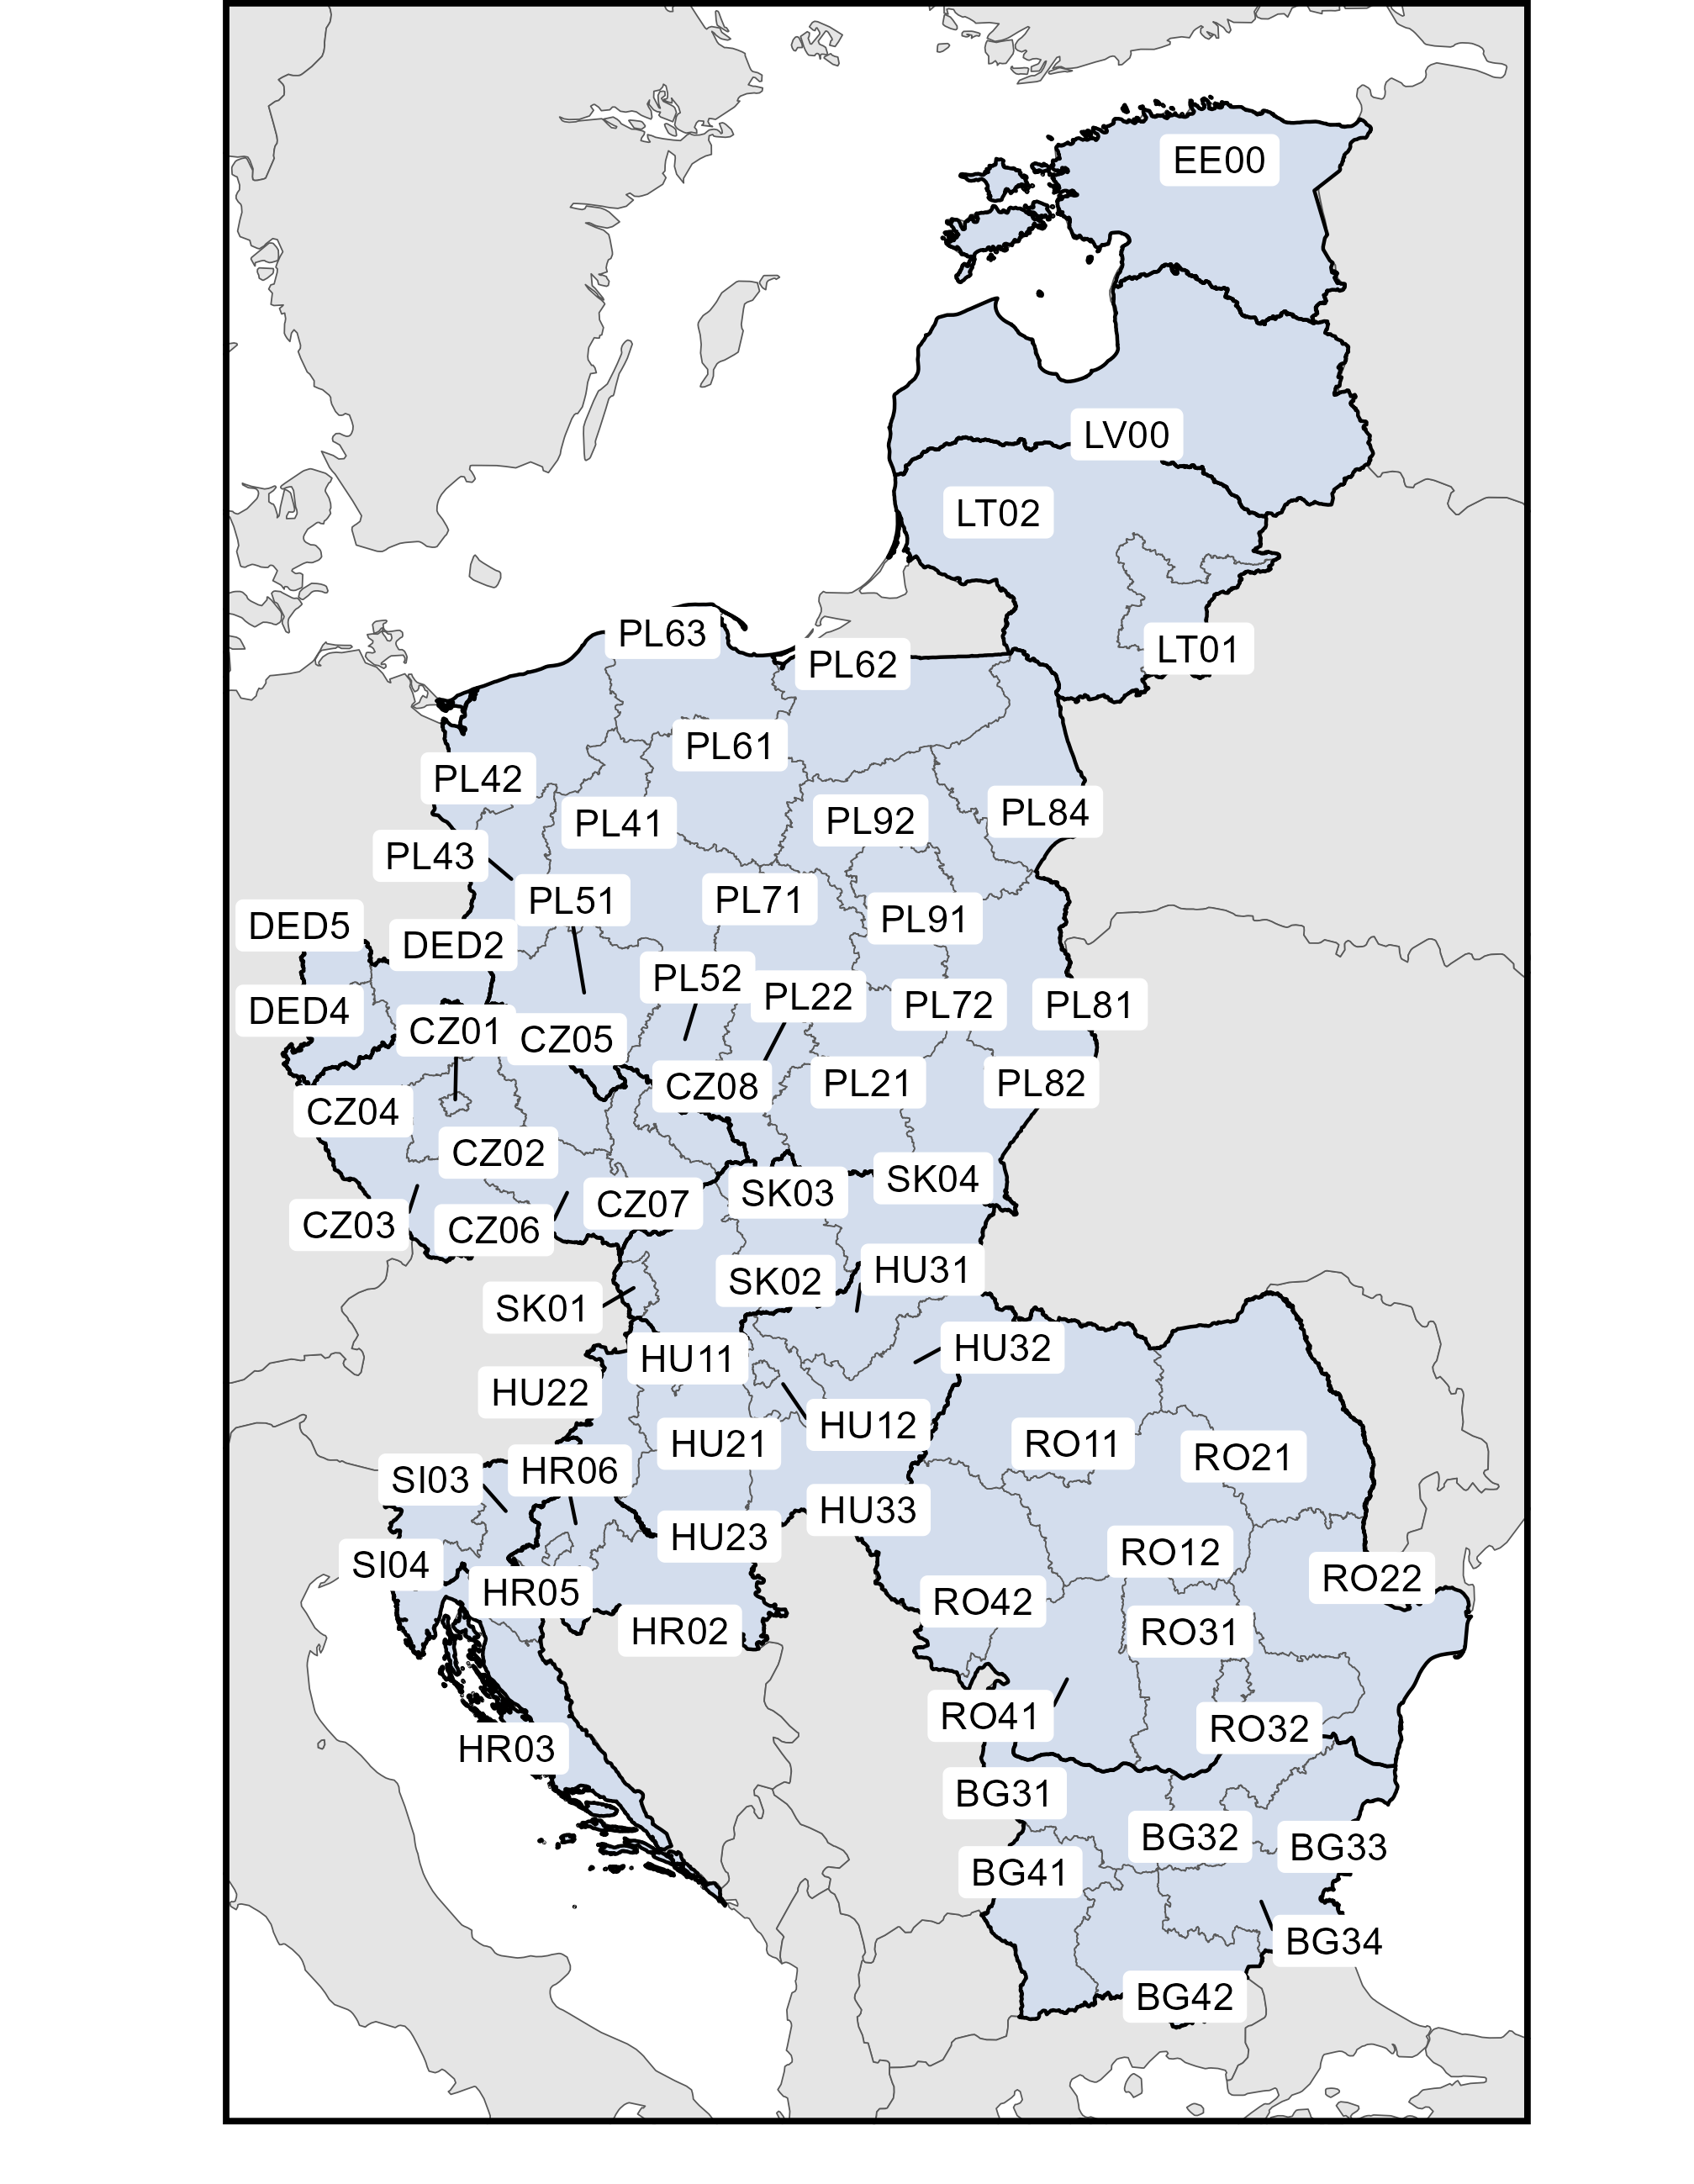
\includegraphics[width=\textwidth]{NUTS_Systematik}
	\begin{spacing}{1} \scriptsize
		Quelle: Eurostat (2024); Dar. imreg (2024) \end{spacing}
\end{figure}


